%\documentclass[oneside,12pt]{Classes/CUEDthesisPSnPDF}
%\documentclass[a4paper]{report}
\documentclass[a4paper,11pt]{report}
\usepackage[hmargin=2cm,vmargin=3cm,bindingoffset=1cm]{geometry}
%\usepackage{suthesis-2e}

\usepackage{setspace}
\usepackage{graphicx}
\usepackage{subfigure}
\usepackage{amsfonts}
\usepackage{amsmath}
\usepackage[algoruled,vlined]{algorithm2e}
\usepackage{listings}
\usepackage{fancyhdr} 
\usepackage{pdfpages}

%%% Fancy Header %%%%%%%%%%%%%%%%%%%%%%%%%%%%%%%%%%%%%%%%%%%%%%%%%%%%%%%%%%%%%%%%%%
% Fancy Header Style Options
\pagestyle{fancy}                       % Sets fancy header and footer
\fancyfoot{}                            % Delete current footer settings
\renewcommand{\chaptermark}[1]{         % Lower Case Chapter marker style
  \markboth{\chaptername\ \thechapter.\ #1}{}} %
\renewcommand{\sectionmark}[1]{        % Lower case Section marker style
  \markright{\thesection.\ #1}}         %
\fancyhead[LE,RO]{\bfseries\thepage}    % Page number (boldface) in left on even
                                        % pages and right on odd pages
\fancyhead[RE]{\bfseries\leftmark}      % Chapter in the right on even pages
\fancyhead[LO]{\bfseries\rightmark}     % Section in the left on odd pages
\renewcommand{\headrulewidth}{0.3pt}    % Width of head rule



\pdfminorversion=5
\pagestyle{headings}
%\linespread{1.5}
\doublespacing
\raggedbottom
\begin{document}

\title{Fast Level Set Segmentation of Biomedical Images using Graphics Processing Units}
\author{Hormuz~Mostofi \\ Keble College\\ \\ \\ \\ \\\\\\\\\\\\\\\\\ \\ \\Department of Engineering Science  \\ Honour School of Engineering, Economics and Management}
%\date{\today}
\maketitle


\includepdf{images/declaration.pdf}
%\begin{acknowledgements} 
%I would like to thank Julia Schnabel and Vicente Grau for their assistance in teaching me about the inner workings of %level set methods. I would also like to thank Daniel Goodman for his guidance in CUDA programming.
%\end{acknowledgements}

\setcounter{tocdepth}{1}
\begin{spacing}{1.2}
\tableofcontents
\end{spacing}


\chapter{Introduction}

\section{Image Segmentation}
Image segmentation is the task of splitting a digital image into one or more regions of interest. It is a fundamental problem in computer vision and many different methods, each with their own advantages and disadvantages, exist for the task. Image segmentation is a particularly difficult task for several reasons. Firstly, the ambiguous nature of splitting up images into objects of interest provides a trade off between making algorithms more generalized or having many user specified parameters. Secondly, imaging artificats such as noise, inhomogeneities, acquisition artifacts and poor contrast, are very difficult to account for in segmentation algorithms without a high level of interactivity from the user. 

In this report, segmentation is discussed in a medical imaging context however the proposed algorithm could equally be used in general purpose segmentations. Segmented images are typically used as the input for applications such as classification, shape analysis and measurement. In medical image processing, segmented images are used for studying anatomical structures, diagnosis and assisting in surgical planning.

Image segmentation also encompasses three dimensional volume segmentations, which are slower to compute by an order of magnitude. It should be noted that before such algorithms existed, segmentation of medical images was done by hand by experts. This was a very accurate, yet slow, process. These segmentations will form the gold standard with which to compare algorithmic segmentations.

In this report, the level set method is used for the purposes of segmentation. Their principal disadvantage is that they are relatively slow to compute, which provides the motivation for optimizing and accelerating such algorithms using graphics processing units (GPUs). Section \ref{upwinding} discusses this further.



\section{Parallel Processing}
The algorithms for processing level sets have vast parallelization potential. Section \ref{levelsetalgorithm} details the algorithms used to discretize the level set equation and Section \ref{parallel} dicusses how these can be executed on graphics hardware.
	\subsection{GPGPU}
General purpose computation on graphics processing units (GPGPU) is the technique of using graphics hardware to compute applications typically handled by the central processing unit (CPU). Graphics cards over the past two decades have been required to become highly efficient at rendering increasingly complex 3D scenes at high frame rates. This has forced their architecture to be massively parallel in order to be compute graphics faster than general purpose CPUs.

Compared to a CPU, a GPU features many more transistors on the control path due to the lower number of control instructions required. Memory is optimized for throughput and not latency, with strict access patterns. GPUs are not optimized for general purpose programs, and does not have the complex instruction sets, or branch control of the modern CPU. It should be noted however that modern CPUs feature multiple cores in order to take advantage of parallel processing. 

The advent of GPGPU programming came with programmable shader units that allowed applying small programs to each pixel or vertex in the rendering pipeline. In order to write code to program the shader units, shading languages had to be used in conjunction with graphics APIs such as DirectX and OpenGL. NVIDIA developed the high-level shading language Cg to assist in programming shaders, however it still required knowledge of graphics APIs. More recently, languages have been developed that allow the programmer to implement algorithms without any knowledge of graphics APIs or architectures. One such language is NVIDIA CUDA, and is the language chosen for the optimizations in this project.

	\subsection{CUDA}
Compute Unified Device Architecture, or CUDA, is NVIDIA's GPGPU technology that allows for programming of the GPU without any graphics knowledge. The C language model has at its core three key abstractions, from \cite{cuda}: a heirarchy of thread groups. shared memories, and barrier synchronization. This breaks the task of parallelization into three sub problems, which allows for language expressivity when threads cooperate, and scalability when extended to multiple processor cores.

		\subsubsection{Framework}
CUDA uses extends C by allowing a programming to write \textit{kernels} that when invoked execute a thousands of lightweight identical threads in parallel. CUDA arranges these threads into a hierarchy of blocks and grids, as can be seen in Figure \ref{fig:cudathreads} allowing for runtime transparent scaling of code to different GPUs. The threads are identified by their location within the grid and block, making CUDA perfectly suited for tasks such as image processing where each threads is easily assigned to an individual pixel or voxel.

\begin{figure}[p]
	\centering
		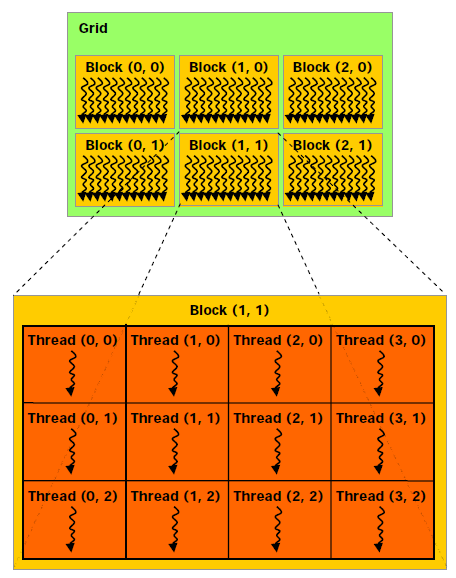
\includegraphics[scale=0.4]{images/cudathreads.PNG}
		\caption{A grid of thread blocks. This figure is taken from \cite{cuda}}
	\label{fig:cudathreads}
\end{figure}

When writing and optimizing complex parallel code in CUDA it is often found that threads may need to cooperate. The memory hierarchy of CUDA threads is shown in Figure \ref{fig:cudamemory}. Here it can be seen that each thread has access to: a per-thread private local memory, a per-block on-chip shared memory to share data between threads, and finally an off-chip global memory accessible to all threads within all blocks. There are also constant and texture memory spaces accessible to all threads, however these are not featured in our algorithm and so will not be discussed in any further detail.

\begin{figure}[p]
	\centering
		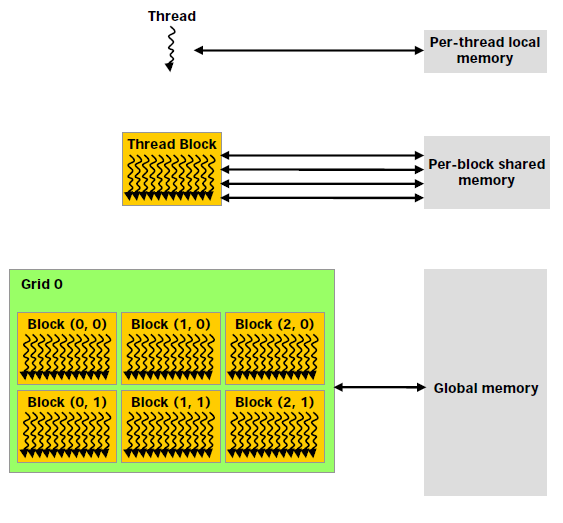
\includegraphics[scale=0.4]{images/cudamemory.PNG}
		\caption{The memory hierarchy of CUDA threads and blocks. This figure is taken from \cite{cuda}}
	\label{fig:cudamemory}
\end{figure}

		\subsubsection{Performance Guidelines}
There are many techniques to optimize a parallel algorithm. Firstly, the optimum block and grid sizes should be used to ensure maximum `occupancy'. Occupancy is the ratio of the number of active warps (32 parallel threads) to the maximum number of active warps supported by the GPU multiprocessor. To maximise efficiency, there is a trade off between making the occupancy very high, ensuring no multiprocessor is ever idle, and making it low enough to ensure no bank conflicts.

Secondly, one of the best ways in which to optimize the parallelization is through efficient memory usage. The global memory space is not cached and therefore has a much higher latency and lower bandwidth than on-chip shared memory. Therefore it is the aim of the programmer to minimise global memory accesses. From \cite{cuda}, it recommended that each thread in a block firstly loads data from global memory to shared memory, synchronizes with all other threads within the thread block to ensure shared memory locations have been written to, processes the data, synchronizes again to ensure shared memory has been fully updated with results, and finally writes the results back to global memory coalesced.

\textit{Coalescence} is an important concept in memory management as it can speed up memory reads and stores significantly. \cite{cuda} lists the following three conditions for coalescing: ``threads must access either 32-bit words, 64-bit words, or 128-bit words'', ``all 16 words must lie in the same segment of size equal to the memory transaction size'' and ``threads must access the words in sequence''. Devices of higher \textit{compute capability} feature incremental improvements to the core architecture, such as more relaxed requirements for coalescence (or support for double-precision floating point accuracy).
\chapter{Method}

In this section, we introduce the level set method and dynamic implicit surfaces. Their role in segmentation is discussed having introduced and defined mathematical constructs such as signed distance transforms.

\section{Level Set Method}\label{levelsetmethod}
The level set method evolves a contour (in two dimensions) or a surface (in three dimensions) implicitly by manipulating a higher dimensional function, called the level set function $\phi(\textbf{x,t})$. The evolving contour or surface can be extracted from the zero level set $\Gamma(\textbf{x,t})=\left\{\phi(\textbf{x,t}) = \textbf{0}\right\}$. The advantage of using this method is that topological changes such as merging and splitting of the contour or surface are catered for implicitly, as can be seen below in Figure \ref{fig:levelsets}. The level set method, since its introduction by Osher and Sethian in \cite{oshersethian}, has seen widespread application in image processing, computer graphics (surface reconstructions) and physical simulation (particularly fluid simulation).

	\begin{figure}[h]
		\centering
			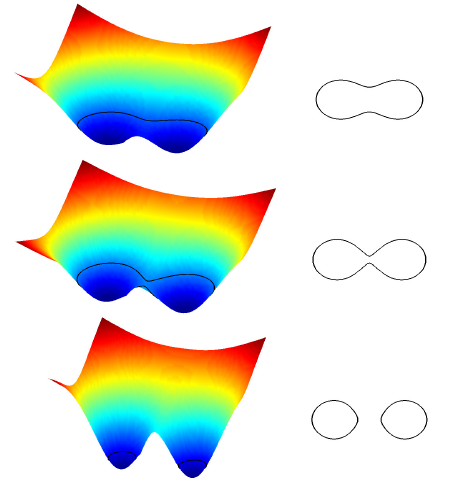
\includegraphics[scale=0.4]{images/levelsets.png}
		\caption{The relationship between the level set function (left) and contour (right) can be seen. It can be seen evolving the surface splits the contour.}
		\label{fig:levelsets}
	\end{figure}

The evolution of the contour or surface is governed by a level set equation. The solution tended to by this partial differential equation is computed iteratively by updating $\phi$ at each time interval. The general form of the level set equation is shown below.

	\begin{equation}
	\frac{\partial{\phi}}{\partial{t}}=-|\nabla{\phi|}\cdot F
	\label{eq:levelsetequation}
	\end{equation}

In the above level set equation $F$ is the velocity term that describes the level set evolution. By manipulating $F$, we can guide the level set to different areas or shapes, given a particular initialization of the level set function. 

\section{Segmentation using Level Sets}\label{thresholding}
Typically, for applications in image segmentation $F$ is dependent on the pixel intensity or curvature values of the level set. The importance of having a curvature term is shown in Figure \ref{leaking}. Here there is no force to smoothen high curvatures, resulting in the contour \textit{leaking}. This is when the level set surface evolves through a anatomical boundary into another anatomical object that was not intended to be segmented. This also makes segmentation difficult for objects which have very high curvature as the curvature weighting term often needs to be set very low in order to allow for these high curvatures, yet doing so may result in such leaking.

\begin{figure}[h]
	\centering
		\subfigure{\includegraphics[scale=0.5]{images/leaking.png}}
		\subfigure{\includegraphics[scale=0.5]{images/leaking2.png}}
	\caption{Leaking when there is no curvature term (or $\alpha = 1$)}
	\label{leaking}
\end{figure}

$F$ may also be dependent on an edge indicator function, which is defined as having a value zero on an edge, and non-zero otherwise. This causes $F$ to slow the level set evolution when on an edge.

In \cite{Lefohn04astreaming} $F$ is dependent on data and curvature functions only (with a weighting parameter between the two) for the purposes of image segmentation. Therefore, we will adopt the same methodology making the level set equation take the form

	\begin{equation}
	\frac{\partial{\phi}}{\partial{t}}=-|\nabla{\phi}|\left[\alpha D(I)  + (1-\alpha)\nabla \cdot{\frac{\nabla{\phi}}{|\nabla{\phi|}}}\right]
	\label{eq:fulllevelsetequation}
	\end{equation}

where the data function $D(I)$ tends the solution towards targeted features, and the mean curvature term $\nabla \cdot{(\nabla{\phi}/|\nabla{\phi|})}$ keeps the level set function smooth. Weighting between these two is $\alpha \in [0,1]$, a free parameter that is set beforehand to control how smooth the contour or surface should be.

The data function $D(I)$ acts as the principal `force' that drives the segmentation. By making $D$ positive in desired regions or negative in undesired regions, the model will tend towards the segmentation sought after. A simple speed function that fulfills this purpose, used by Lefohn, Whitaker and Cates in \cite{Lefohn04astreaming, gist}, is given by

	\begin{equation}
	D(I)= \epsilon - |I-T|
	\label{eq:dataterm}
	\end{equation}

which is plotted in Figure \ref{fig:speedterm}. Here $T$ describes the central intensity value of the region to be segmented, and $\epsilon$ describes the intensity deviation around T that is part of the desired segmentation. Therefore if a pixel or voxel has an intensity value within the $T\pm\epsilon$ range the model will expand, and otherwise it will contract. 

	\begin{figure}[h]
		\centering
			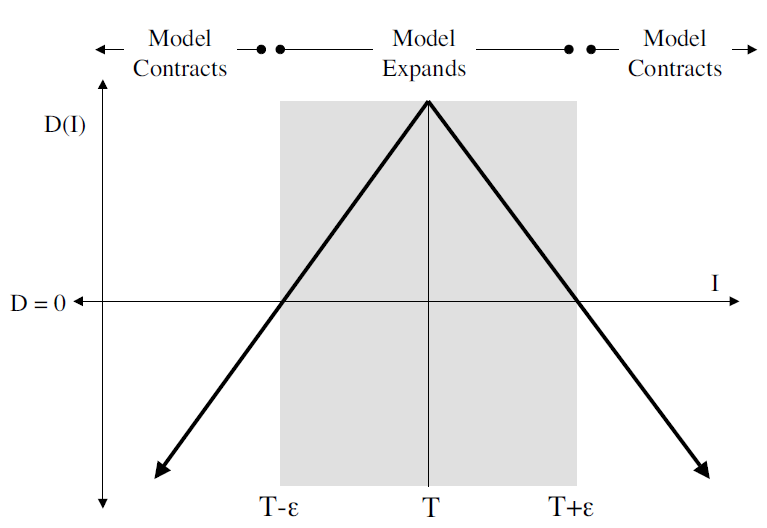
\includegraphics[scale=0.3]{images/speedterm.png}
		\caption{The speed term from \cite{gist}}
		\label{fig:speedterm}
	\end{figure}

Therefore the three user parameters that need to be specified for segmentation are $T$,$\epsilon$ and $\alpha$. An initial mask (to be transformed to a signed distance function as discussed in Section \ref{sdf}) for the level set function is also required, which may take the form of a cube in three dimensions or a square in two dimensions, or any other arbitrary closed shape. Typically, the user selects spherical seed points specifying the center in $i,j,k$ space and the radius to guide the level set to the anatomical object of interest.

The level set iteration can be terminated once $\phi$ has converged, or after a certain number of iterations. 


	\subsection{Signed Distance Transforms}\label{sdf}
A distance transform assigns a value for every pixel (or voxel) within a binary image containing one or more objects a value which represents the minimum distance from that pixel to the closest pixel on the boundary of the object(s). The mathematical definition of a distance function $D:\mathbb{R}^3 \rightarrow \mathbb{R}$ for a set $S$, from \cite{oshersethian}, is
	
	\begin{equation}
	D(r,S) = \textrm{min}{|r-S|} \textrm{ for all } r \in \mathbb{R}^3
	\label{eq:distancetransform}
	\end{equation}

A \textit{signed} distance transform assigns the sign of the distance value as positive for those pixels outside the object, and negative for those inside it. This is the sign convention that will be followed in the implementation, however the opposite sign convention could also be used. It should be noted that the distance values depend on the chosen metric for distance: some common distance metrics are Euclidean distance, chessboard distance, and city block distance. Many of the algorithms that compute signed Euclidean distance transforms (SEDT) often trade accuracy for efficiency and feature varying levels of complexity.

Signed distance transforms are required to initialize $\phi$ and also to reinitialize it every certain number of iterations. Computation of the initialization of $\phi$ is required before iteration of the level set equation can take place, and this will typically be a signed distance transform of an initial mask. Therefore the level set segmentation filter requires two images: an initial mask (which indicates targeted regions) and a \textit{feature} image (which is the image to be segmented). 
The choice of how often to reinitialize is an important one: if the number of iterations between reinitialization is too low the level set will simply oscillate, if it is too high the risky of instabilities is elevated. 
	
	\begin{figure}
	  \begin{center}
	    \subfigure[Arbitrary Initial Mask]{\label{fig:initmask}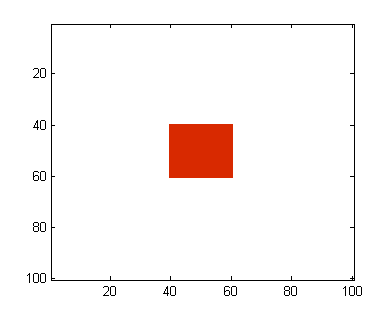
\includegraphics[scale=0.5]{images/initmask.png}}
	    \subfigure[Signed Distance Transform of Mask with Zero Level Set Overlaid]{\label{fig:sdf}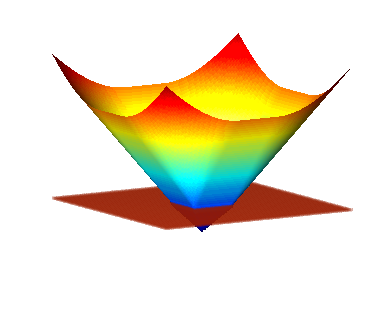
\includegraphics[scale=0.5]{images/sdf.png}}
	  \end{center}
	  \caption{2D Signed Euclidean Distance Transform}
	  \label{fig:sdfexplanation}
	\end{figure}
	
Alternatively, \cite{gui2005lse} provides a method of evolving level sets without reinitialization using signed distance transforms by forcing the level set function to be close to a signed distance function.

	\subsection{3D Volume Segmentations}\label{3dvolumesegmentation}
Extending a two dimensional level set segmentation algorithm to three dimensions is a relatively straightforward task, however requires careful consideration of boundary conditions. There are many more derivatives that are required in order to compute the level set update. In addition to the increased number of variables, creating a signed Euclidean distance function is one of the major challenges in developing 3D segmentation code. Unfortunately, neither C code or CUDA code was available to perform distance transform (re)initialization in 3D and therefore MATLAB was used to initialize and reinitialize the level set during execution. There has however been recent work on CUDA accelerated distance transforms from \cite{difi},\cite{gpgpudistance}.
The storage and computational complexity of 3D volume segmentation must also be appreciated and forms much of the motivation for acceleration with CUDA.
\chapter{Implementation}

\section{Level Set Algorithm}\label{levelsetalgorithm}

\subsection{Upwinding}
Equation \eqref{eq:levelsetequation}, the level set equation, needs to be discretized for both sequential and parallel computation. This is done using the \textit{up-wind} differencing scheme. The following explanation of \textit{upwinding} is from \cite{osher2003lsm}.

A first order accurate method for time discretization of equation \eqref{eq:levelsetequation}, is given by the forward Euler method, from \cite{osher2003lsm}:

\begin{equation}
\frac{\phi^{t+\Delta t}-\phi^t}{\Delta t} +F^{t}\cdot{\nabla{\phi^{t}}} = 0
\label{eq:euler1}
\end{equation}

where $\phi^{t}$ represents the current values of $\phi$ at time $t$, $F^{t}$ represents the velocity field at time $t$, and  $\nabla{\phi^{t}}$ represents the values of the gradient of $\phi$ at time $t$. When computing the gradient, a great deal of care must be taken with regards to the spatial derivatives of $\phi$. This is best exemplified by considering the expanded form of equation \eqref{eq:euler1}.

\begin{equation}
\frac{\phi^{t+\Delta t}-\phi^t}{\Delta t} +u^{t}\phi_x^t+v^{t}\phi_y^t+w^{t}\phi_z^t = 0
\label{eq:euler2}
\end{equation}

For simplicity, consider the one dimensional form of equation \eqref{eq:euler2} at a specific grid point $x_i$ 

\begin{equation}
\frac{\phi^{t+\Delta t}-\phi^t}{\Delta t} +u_i^{t}(\phi_x)_i^t = 0
\label{eq:euler3}
\end{equation}

where $(\phi_x)_i$ is the spatial derivative of $\phi$ at $x_i$. The method of characteristics indicates whether to use a forward difference or backwards difference for $\phi$ based on the sign of $u_i$ at the point $x_i$. If $u_i > 0$, the values of $\phi$ are moving from left to right, and therefore backwards difference methods ($D_x^-$) should be used. Conversely, if $u_i<0$, forward difference methods ($D_x^+$) should be used to approximate $\phi_x$. It is this process of choosing which approximation for the spatial derivative of $\phi$ to use based on the sign of $u_i$ that is known as \textit{upwinding}. 

Extending this to three dimensions, from \cite{Lefohn04astreaming}, results in the derivatives below required for the level set equation update. 

\begin{eqnarray}
	D_x &=& (u_{i+1,j,k}-u_{i-1,j,k})/2 \nonumber\\
	D_y &=& (u_{i,j+1,k}-u_{i,j-1,k})/2 \nonumber\\
	D_z &=& (u_{i,j,k+1}-u_{i,j,k-1})/2 \nonumber\\
	D_x^+ &=& u_{i+1,j,k}-u_{i,j,k} \nonumber\\
	D_y^+ &=& u_{i,j+1,k}-u_{i,j,k} \nonumber\\
	D_z^+ &=& u_{i,j,k+1}-u_{i,j,k} \nonumber\\
	D_x^- &=& u_{i,j,k}-u_{i-1,j,k} \nonumber\\
	D_y^- &=& u_{i,j,k}-u_{i,j-1,k} \nonumber\\
	D_z^- &=& u_{i,j,k}-u_{i,j,k-1} \nonumber\\
\end{eqnarray}

$\nabla\phi$ is approximated using the upwind scheme.

\begin{eqnarray}
\nabla\phi_{max} &=& \left[
  \begin{array}{ c }
     \sqrt{max(D_x^+, 0)^2 + max(-D_x^+,0)^2}  \\[2em]
     \sqrt{max(D_y^+, 0)^2 + max(-D_y^+,0)^2}  \\[2em]
     \sqrt{max(D_z^+, 0)^2 + max(-D_z^+,0)^2}  
  \end{array} \right] \\[2em]
\nabla\phi_{min} &=& \left[
  \begin{array}{ c }
     \sqrt{min(D_x^+, 0)^2 + min(-D_x^+,0)^2}  \\[2em]
     \sqrt{min(D_y^+, 0)^2 + min(-D_y^+,0)^2}  \\[2em]
     \sqrt{min(D_z^+, 0)^2 + min(-D_z^+,0)^2} 
  \end{array} \right] 
\end{eqnarray}

Finally, depending on whether $F_{i,j,k} > 0$ or $F_{i,j,k} < 0$, $\nabla\phi$ is 

\begin{equation}
\nabla\phi = \left\{ 
\begin{array}{l l}
  ||\nabla\phi_{max}||_2 & \quad \mbox{if $F_{i,j,k} > 0$}\\
  ||\nabla\phi_{min}||_2 & \quad \mbox{if $F_{i,j,k} < 0$}\\ \end{array} \right.
\label{eq:finalchoice}
\end{equation}

\begin{equation}
\phi(t+\Delta t) =\phi(t) + \Delta t F|\nabla\phi|
\label{eq:phi}
\end{equation}

The speed term $F$, as discussed before, is based on the pixel intensity values and curvature values. 

\subsection{Curvature}
Curvature is computed based on the values of the current level set using the derivatives below. In two dimensions only the first two derivatives are required, alongside the derivatives defined previously. In three dimensions, all the derivatives below are required.

\begin{eqnarray}
	D_x^{+y} &=& (u_{i+1,j+1,k}-u_{i-1,j+1,k})/2 \nonumber\\
	D_x^{-y} &=& (u_{i+1,j-1,k}-u_{i-1,j-1,k})/2 \nonumber\\
	D_x^{+z} &=& (u_{i+1,j,k+1}-u_{i-1,j,k+1})/2 \nonumber\\
	D_x^{-z} &=& (u_{i+1,j,k-1}-u_{i-1,j,k-1})/2 \nonumber\\
	D_y^{+x} &=& (u_{i+1,j+1,k}-u_{i+1,j-1,k})/2 \nonumber\\
	D_y^{-x} &=& (u_{i-1,j+1,k}-u_{i-1,j-1,k})/2 \nonumber\\
	D_y^{+z} &=& (u_{i,j+1,k+1}-u_{i,j-1,k+1})/2 \nonumber\\
	D_y^{-z} &=& (u_{i,j+1,k-1}-u_{i,j-1,k-1})/2 \nonumber\\
	D_z^{+x} &=& (u_{i+1,j,k+1}-u_{i+1,j,k-1})/2 \nonumber\\
	D_z^{-x} &=& (u_{i-1,j,k+1}-u_{i-1,j,k-1})/2 \nonumber\\
	D_z^{+y} &=& (u_{i,j+1,k+1}-u_{i,j+1,k-1})/2 \nonumber\\
	D_z^{-y} &=& (u_{i,j-1,k+1}-u_{i,j-1,k-1})/2 \nonumber\\
\end{eqnarray}

Using the \textit{difference of normals} method from \cite{Lefohn04astreaming}, curvature is computed using the above derivates with the two normals $\textbf{n}^+$ and $\textbf{n}^-$.

\begin{eqnarray}
\textbf{n}^+ &=& \left[
  \begin{array}{ c }
     \frac{D_x^+}{\sqrt{(D_x^+)^2 + {\left(\frac{D_y^{+x}+D_y}{2}\right)}^2 +{\left(\frac{D_z^{+x}+D_z}{2}\right)}^2  }}  \\[2em]
     \frac{D_y^+}{\sqrt{(D_y^+)^2 + {\left(\frac{D_x^{+y}+D_x}{2}\right)}^2 +{\left(\frac{D_z^{+y}+D_z}{2}\right)}^2  }}  \\[2em]
     \frac{D_z^+}{\sqrt{(D_z^+)^2 + {\left(\frac{D_y^{+z}+D_x}{2}\right)}^2 +{\left(\frac{D_y^{+z}+D_y}{2}\right)}^2  }}  
  \end{array} \right] \\[2em]
\textbf{n}^- &=& \left[
  \begin{array}{ c }
     \frac{D_x^-}{\sqrt{(D_x^-)^2 + {\left(\frac{D_y^{-x}+D_y}{2}\right)}^2 +{\left(\frac{D_z^{-x}+D_z}{2}\right)}^2  }}  \\[2em]
     \frac{D_y^-}{\sqrt{(D_y^-)^2 + {\left(\frac{D_x^{-y}+D_x}{2}\right)}^2 +{\left(\frac{D_z^{-y}+D_z}{2}\right)}^2  }}  \\[2em]
     \frac{D_z^-}{\sqrt{(D_z^-)^2 + {\left(\frac{D_y^{-z}+D_x}{2}\right)}^2 +{\left(\frac{D_y^{-z}+D_y}{2}\right)}^2  }}  
  \end{array} \right] 
\end{eqnarray}

The two normals are used to compute divergence, allowing for mean curvature to be computed as shown below in equation \eqref{eq:curv}.

\begin{equation}
H = \frac{1}{2}\nabla\cdot\frac{\nabla\phi}{|\nabla\phi|} = \frac{1}{2}((\textbf{n}_x^+ - \textbf{n}_x^-)+(\textbf{n}_y^+ - \textbf{n}_y^-)+(\textbf{n}_z^+ - \textbf{n}_z^-))
\label{eq:curv}
\end{equation}

\subsection{Stability}
From \cite{osher2003lsm}, a finite difference approximation to a linear partial differential equation is convergent if and only if it is both consistent and stable. Stability implies that small errors in the solution are not amplified during iteration. Stability is enforced using the Courant-Friedreichs-Lewy (CFL) condition which states the numerical wave speed must be greater than the physical wave speed, i.e. $\Delta x/\Delta t>|u|$. Rearranging, we have

\begin{equation}
\Delta t < \frac{\Delta x}{max\left\{|u|\right\}}
\label{eq:cfl}
\end{equation}

which is usually implemented, through variants of equation \eqref{eq:cfl}, by choosing a \textit{CFL number} that lies between 0 and 1 to further guarentee stability.

\section{Sequential Implementation}

	\subsection{Matlab}
The first task was to write code in MATLAB to segment two dimensional greyscale images. The MATLAB Image Processing Toolbox provides many functions (such as to load, resample and filter images, compute distance transforms and easily visualise the level set evolution) which kept the code reasonably concise. 

The code is split into two files, in order to seperate the initialisation and level set update code

	\subsection{C}

\section{Parallel Implemention}
	\subsection{Block and Grid Sizes}
	\subsection{Shared Memory}
\chapter{Results}
	\section{Speed Tests and Analysis}
	\section{Limitations}
	

\chapter{Conclusions and Future Work}
\section{Conclusion}
In this project report a fast segmentation algorithm has been presented and analysed. The implementation on the graphics device is very fast, with large two dimensional images and three dimensional volumes segmented $30$ to $40$ times faster (on a relatively low performance GPU) than sequential algorithms. 
The method of using level sets to segment images, and how to accelerate this process using GPUs has been discussed in great detail. The numerical methods used for the implementation were listed in Section \ref{levelsetalgorithm}. Giles' CUDA kernel for laplace discretization in 3D \cite{mgiles} has been adapted for level set iteration. In Section \ref{results} it was seen that the power of GPU acceleration was demonstrated for very large data sets.

Given the wide range of applications level sets have in computing (image processing, computer graphics and physical simulation) this algorithm serves as an excellent framework to solve a diverse array of problems.
	
CUDA itself has been shown to be an excellent framework to accelerate computational problems in engineering, and is gaining more features and fewer limitations every few months. The principal disadvantages of CUDA are that it is only effective for very data parallel problems, and that it is not an industry standard. Recently, to counter the latter, it is very likely that it will in fact be replaced by \textit{OpenCL} (Open Computing Language). The syntax and architecture between CUDA and OpenCL will be very similar, allowing this code to be easily ported to OpenCL.

\section{Future Work}
There are several areas in which this algorithm could be improved which revolve around three central themes of speed, accuracy and usability. 

In terms of speed, integrating the narrow band method into the algorithm will provide significant further speed up, however increases the complexity of the kernel (potentially resulting in higher register usage and therefore less occupancy). Secondly, adding support for multiple GPUs and testing on very high performance hardware would be of significant interest. 

Including a 3D signed Euclidean distance transform function is very important for volume segmentation. This would need to be implemented in CUDA in order to prevent costly transfers of data from the device to the host. To increase accuracy, integrating filters in CUDA to preprocess the medical data is strongly encouraged. Including more terms into the level set speed function (such as edge stopping functions) would allow the algorithm to segment unhomogenous gray valued regions. 

Finally, in order to make the segmentation more interactive and versatile, it is suggested to include a graphical user interface allowing segmentation to be visualized and guided at the same time. In order to ensure visualization does not affect performance it is suggested to use two GPUs: one to process the level set and the other to render the level set evolution.

\begin{spacing}{1.2}
\chapter{Appendix}


\section{MATLAB Level Set Update Code}
\lstinputlisting{simpleseg.m}





\bibliographystyle{plain}
\bibliography{References}
\end{spacing}

\includepdf[landscape]{images/riskassess.pdf}

\end{document}